
\documentclass[11pt]{article}
\usepackage[notes]{la}
\lamodule{1}{1}{Systems of Linear Equations}
 
\begin{document}
 
\section{Systems of Linear Equations}
 
\begin{remark}[How to read these notes]
These notes are meant to be read \emph{actively}. Besides definitions, theorems and worked
examples, you will meet three kinds of prompts.
\begin{itemize}
  \item A \textbf{Knowledge Check} is a short question that you should be able to answer right
        after reading the preceding paragraph. Try it \emph{before} looking at its answer at the
        end of the section.
  \item A \textbf{Pause and think} box is a deeper question with no one-line answer. These are about
        \emph{why}, not \emph{how}. Discuss them with a neighbor first; a complete discussion of each
        one appears in the answers at the end of the section, numbered to match.
  \item A \textbf{Warning} flags a common mistake so that you can avoid it.
\end{itemize}
Every theorem is either proved or you are told exactly where its proof will be supplied.
The goal is not only that you can row reduce a matrix, but that you can explain
\emph{why} the method works and \emph{what} its output means.
\end{remark}
 
\begin{guide}
A system of equations is a list of constraints that must hold \emph{simultaneously}. Before
doing a lot of computation: how can we tell whether any assignment of values satisfies all the
constraints? And if one does, is it the only one?
\end{guide}
 
\textbf{By the end of this section you should be able to:}
\begin{itemize}
  \item decide whether an equation is linear, and whether a list of numbers solves a system;
  \item describe the three possible sizes of a solution set and explain why no other size occurs;
  \item translate a system into an augmented matrix and back;
  \item use the three elementary row operations, and explain why they never change the solution set;
  \item recognize an inconsistent system from the row it produces.
\end{itemize}
 
% ---------------------------------------------------------------------
\subsection*{Linear equations}
 
\begin{defn}{Linear equation}{lineq}
A \emph{linear equation} in the variables $x_1,\dots,x_n$ is an equation that can be written in
the form
\[
a_1x_1+a_2x_2+\cdots+a_nx_n=b,
\]
where $b$ and the \emph{coefficients} $a_1,\dots,a_n$ are real numbers known in advance.
The number of variables $n$ can be any positive integer.
\end{defn}
 
``Linear'' is a statement about how the \emph{unknowns} appear: each unknown is multiplied by a
constant, and the results are added. An equation does not have to \emph{look} like the
form above; it only has to be rearrangeable into it. For example,
\[
x_2 = 2(3-x_1)+x_3 \quad\text{rearranges to}\quad 2x_1+x_2-x_3=6,
\]
so it is linear. On the other hand,
\[
x_1x_2=4,\qquad x_1+\sqrt{x_2}=1,\qquad x_1^2+x_2=0
\]
are not linear: they contain a product of unknowns, a square root of an unknown, and a square.
 
\begin{kc}{Is it linear?}{linear}
Decide which of the following are linear equations in $x_1,x_2,x_3$.
\begin{enumerate}[label=(\alph*)]
  \item $3x_1-x_2=7$
  \item $x_1x_3+x_2=1$
  \item $\tfrac12 x_1+\pi x_2=4$
  \item $x_1^2+x_2=0$
  \item $5=2x_2-3x_1$
\end{enumerate}
\end{kc}
 
\begin{think}{Lines versus curves}{lines}
In two variables, $ax_1+bx_2=c$ graphs as a line, while $x_1x_2=4$ graphs as a hyperbola.
A line and a hyperbola can meet in exactly two points. Keep this in mind: later in this
section you will be asked to explain why \emph{two lines} can never meet in exactly two points.
What property of lines is the hyperbola missing?
\end{think}
 
% ---------------------------------------------------------------------
\subsection*{Systems and solutions}
 
\begin{defn}{System, solution, solution set}{system}
A \emph{system of linear equations} (or \emph{linear system}) is a collection of one or more
linear equations in the \emph{same} variables $x_1,\dots,x_n$.
 
A \emph{solution} of the system is a list $(s_1,\dots,s_n)$ of numbers that makes \emph{every}
equation in the system a true statement when $s_1,\dots,s_n$ are substituted for
$x_1,\dots,x_n$. The set of all solutions is the \emph{solution set}. Two systems are
\emph{equivalent} if they have the same solution set.
\end{defn}
 
For example, consider
\begin{equation}\label{eq:2x2}
\begin{aligned}
x_1+2x_2&=5\\
3x_1-x_2&=1.
\end{aligned}
\end{equation}
The list $(1,2)$ is a solution: $1+2\cdot2=5$ and $3\cdot1-2=1$. The word ``every'' in the
definition matters. A list that satisfies only some of the equations is \emph{not} a solution.
 
\begin{kc}{Checking a candidate}{candidate}
Is $(3,1)$ a solution of system \eqref{eq:2x2}? Show the substitution.
\end{kc}
 
% ---------------------------------------------------------------------
\subsection*{How many solutions can a system have?}
 
With two equations in two unknowns, each equation is a line in the plane and a solution is a
point lying on \emph{both} lines. Lines in the plane can be arranged in three ways.
 
\begin{center}
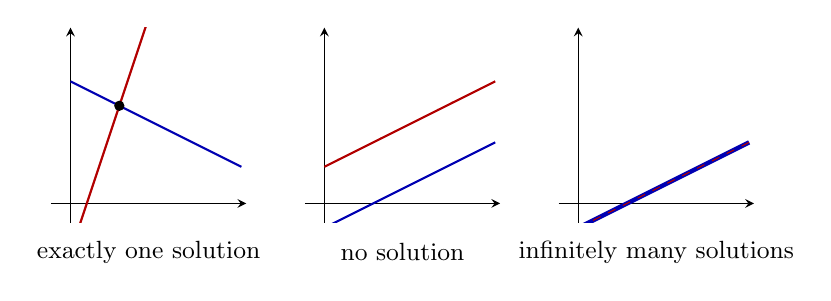
\begin{tikzpicture}[scale=0.62,>=stealth]
\begin{scope}
  \clip (-0.4,-0.4) rectangle (3.6,3.6);
  \draw[->] (-0.4,0)--(3.6,0); \draw[->] (0,-0.4)--(0,3.6);
  \draw[thick,blue!70!black,domain=0:3.5] plot (\x,{(5-\x)/2});
  \draw[thick,red!70!black,domain=0:3.5] plot (\x,{3*\x-1});
  \fill (1,2) circle (3pt);
\end{scope}
\node at (1.6,-1.0) {\small exactly one solution};
\begin{scope}[xshift=5.2cm]
  \clip (-0.4,-0.4) rectangle (3.6,3.6);
  \draw[->] (-0.4,0)--(3.6,0); \draw[->] (0,-0.4)--(0,3.6);
  \draw[thick,blue!70!black,domain=0:3.5] plot (\x,{(\x-1)/2});
  \draw[thick,red!70!black,domain=0:3.5] plot (\x,{\x/2+0.75});
\end{scope}
\node at (6.8,-1.0) {\small no solution};
\begin{scope}[xshift=10.4cm]
  \clip (-0.4,-0.4) rectangle (3.6,3.6);
  \draw[->] (-0.4,0)--(3.6,0); \draw[->] (0,-0.4)--(0,3.6);
  \draw[ultra thick,blue!70!black,domain=0:3.5] plot (\x,{(\x-1)/2});
  \draw[thin,red!70!black,dashed,domain=0:3.5] plot (\x,{(\x-1)/2});
\end{scope}
\node at (12.0,-1.0) {\small infinitely many solutions};
\end{tikzpicture}
\end{center}
 
The three pictures correspond to system \eqref{eq:2x2} (the lines cross at $(1,2)$);
to $x_1-2x_2=1,\ {-2x_1}+4x_2=3$ (parallel lines); and to $x_1-2x_2=1,\ {-2x_1}+4x_2=-2$ (the
second equation is $-2$ times the first, so the lines coincide).
 
\begin{defn}{Consistent and inconsistent}{consistent}
A system is \emph{consistent} if it has at least one solution and \emph{inconsistent} if it has
none.
\end{defn}
 
Is it an accident of the picture that we never see exactly two solutions? Not at all.
 
\begin{thm}{Only three possibilities}{three}
A system of linear equations has either no solution, or exactly one solution, or infinitely many
solutions.
\end{thm}
 
\begin{proof}
Suppose the system has two \emph{different} solutions $p=(p_1,\dots,p_n)$ and
$q=(q_1,\dots,q_n)$. We show that it has infinitely many.
For a real number $t$, define the list
\[
r(t)=\bigl((1-t)p_1+tq_1,\ \dots,\ (1-t)p_n+tq_n\bigr).
\]
Take any one equation of the system, $a_1x_1+\cdots+a_nx_n=b$. Substituting $r(t)$ gives
\begin{align*}
a_1\bigl((1-t)p_1+tq_1\bigr)+\cdots+a_n\bigl((1-t)p_n+tq_n\bigr)
&=(1-t)\underbrace{(a_1p_1+\cdots+a_np_n)}_{=\,b}+t\underbrace{(a_1q_1+\cdots+a_nq_n)}_{=\,b}\\
&=(1-t)b+tb=b.
\end{align*}
So $r(t)$ satisfies every equation, i.e.\ $r(t)$ is a solution for \emph{every} real $t$.
Finally, if $t\ne s$, then the $i$th entries of $r(t)$ and $r(s)$ differ by $(t-s)(q_i-p_i)$, and
this is nonzero for some $i$ because $p\ne q$. So different values of $t$ give different
solutions, and there are infinitely many of them.
\end{proof}
 
\begin{think}{Anatomy of the proof}{proof}
\begin{enumerate}[label=(\arabic*)]
  \item Geometrically, what is the set $\{r(t): t\in\R\}$? (Try $n=2$ and $n=3$.)
  \item Where in the proof did we use that the equations are \emph{linear}? Redo the
        computation for $x_1x_2=4$ with $p=(1,4)$ and $q=(4,1)$ and see which step fails.
  \item Use the theorem to explain why two lines in the plane can never meet in exactly two
        points. (This answers the question from the earlier box.)
\end{enumerate}
\end{think}
 
% ---------------------------------------------------------------------
\subsection*{Matrix notation}
 
Writing the variables over and over is wasteful: all of the information in a linear system is
in its coefficients and right-hand sides. We record it in a rectangular array of numbers called a
\emph{matrix}. A matrix with $m$ rows and $n$ columns is an $m\times n$ matrix
(read ``$m$ by $n$''); \textbf{rows are always counted first}.
 
For the system
\begin{equation}\label{eq:3x3}
\begin{aligned}
x_1+\phantom{2}x_2+x_3&=\phantom{-}2\\
2x_1+3x_2+x_3&=\phantom{-}6\\
x_1-\phantom{2}x_2+2x_3&=-1
\end{aligned}
\end{equation}
we line up the variables in columns and obtain
\[
\underbrace{\begin{bmatrix}1&1&1\\2&3&1\\1&-1&2\end{bmatrix}}_{\text{coefficient matrix } (3\times3)}
\qquad
\underbrace{\begin{amat}{ccc|c}1&1&1&2\\2&3&1&6\\1&-1&2&-1\end{amat}}_{\text{augmented matrix } (3\times4)}
\]
The \emph{coefficient matrix} contains only the coefficients; the \emph{augmented matrix}
adds a final column containing the right-hand sides. (The vertical bar is only a visual
reminder of where the equal signs were.) If a variable is missing from an equation, its
coefficient is $0$.
 
\begin{kc}{Matrix to system and back}{augmented}
Write the augmented matrix of
\[
2x_1-x_3=4,\qquad x_2+3x_3=-1,
\]
and state its size. (Be careful about the missing variables.)
\end{kc}
 
% ---------------------------------------------------------------------
\subsection*{Elementary row operations}
 
The strategy for solving a system is to replace it by an \emph{equivalent} system that is easier to
read off. We do this with three operations, written here on the rows of the augmented matrix
(each row is one equation).
 
\begin{defn}{Elementary row operations}{rowops}
\begin{enumerate}[itemsep=2pt]
  \item \textbf{Replacement:} replace row $i$ by the sum of row $i$ and a multiple of a
        \emph{different} row $j$. Notation: $R_i+cR_j\to R_i$.
  \item \textbf{Interchange:} swap two rows. Notation: $R_i\leftrightarrow R_j$.
  \item \textbf{Scaling:} multiply every entry of a row by a \emph{nonzero} constant.
        Notation: $cR_i\to R_i$ ($c\neq0$).
\end{enumerate}
Two matrices are \emph{row equivalent} if one can be turned into the other by a sequence of
elementary row operations. We write $A\sim B$.
\end{defn}
 
Row operations can be applied to \emph{any} matrix, not only an augmented one. But why are
these three operations allowed? Why can we be sure we are not accidentally changing the answer?
 
\begin{thm}{Row operations preserve solutions}{rowsol}
If the augmented matrices of two linear systems are row equivalent, then the two systems have the
same solution set.
\end{thm}
 
\begin{proof}
It is enough to show that a \emph{single} elementary row operation does not change the solution
set; the theorem then follows by repeating the argument for each operation in the sequence.
Let $p$ be a solution of the original system. We check each operation.
\begin{itemize}
  \item \emph{Interchange.} The new system contains exactly the same equations in a different
        order, so $p$ still satisfies all of them.
  \item \emph{Scaling.} If $p$ satisfies $L_i=b_i$, then it satisfies $cL_i=cb_i$ (multiply
        both sides by $c$).
  \item \emph{Replacement.} If $p$ satisfies $L_i=b_i$ and $L_j=b_j$, then it satisfies
        $L_i+cL_j=b_i+cb_j$, which is the new equation. The other equations are unchanged.
\end{itemize}
So every solution of the old system is a solution of the new one. For the converse we use that
every elementary row operation can be \emph{undone} by another elementary row operation:
interchange is undone by the same interchange; scaling by $c\neq0$ is undone by scaling by $1/c$;
and $R_i+cR_j\to R_i$ is undone by $R_i-cR_j\to R_i$. Hence the old system is obtained from
the new one by row operations, and the same argument shows every solution of the new system
is a solution of the old one.
\end{proof}
 
\begin{kc}{Undoing a row operation}{undo}
Name the elementary row operation that undoes each of: (a) $R_3-5R_1\to R_3$;
(b) $R_2\leftrightarrow R_4$; (c) $4R_2\to R_2$.
\end{kc}
 
\begin{think}{Why these restrictions?}{rowops}
\begin{enumerate}[label=(\arabic*)]
  \item The proof needs $c\neq0$ in scaling. What would the operation ``$0\cdot R_i\to R_i$'' do to
        the system, and exactly which step of the proof breaks?
  \item In replacement we insisted that $j\neq i$. What happens if you try
        $R_i+cR_i\to R_i$ with $c=-1$? Why is that not safe, even though it looks like a
        replacement?
  \item Reversibility is the real reason the method is safe. Can you think of an everyday
        ``operation'' on an equation (for example, squaring both sides) that is \emph{not}
        reversible and can therefore introduce false solutions?
\end{enumerate}
\end{think}
 
% ---------------------------------------------------------------------
\subsection*{Worked examples}
 
The plan is to use the leading term of the first equation to eliminate that variable from the
equations below it, then repeat with the next equation, and so on.
 
\begin{exmp}{A system with exactly one solution}{unique}
Solve system \eqref{eq:3x3}.
 
\medskip\textbf{Solution.} Work with the augmented matrix. Use the $1$ in the upper left to clear
the first column below it, then the $1$ in row~2 to clear the second column below it:
\begin{align*}
\begin{amat}{ccc|c}1&1&1&2\\2&3&1&6\\1&-1&2&-1\end{amat}
&\rops{R_2-2R_1,\ R_3-R_1}
\begin{amat}{ccc|c}1&1&1&2\\0&1&-1&2\\0&-2&1&-3\end{amat}
\rops{R_3+2R_2}
\begin{amat}{ccc|c}1&1&1&2\\0&1&-1&2\\0&0&-1&1\end{amat}
\end{align*}
The bottom row now says $-x_3=1$. Scale it, then use it to clear the third column above it,
and finally clear the second column above row~2:
\begin{align*}
&\rops{-R_3}
\begin{amat}{ccc|c}1&1&1&2\\0&1&-1&2\\0&0&1&-1\end{amat}
\rops{R_2+R_3,\ R_1-R_3}
\begin{amat}{ccc|c}1&1&0&3\\0&1&0&1\\0&0&1&-1\end{amat}
\rops{R_1-R_2}
\begin{amat}{ccc|c}1&0&0&2\\0&1&0&1\\0&0&1&-1\end{amat}
\end{align*}
This is the augmented matrix of $x_1=2,\ x_2=1,\ x_3=-1$. By Theorem~\ref{thm:rowsol} this is the
only solution of \eqref{eq:3x3}: $(2,1,-1)$.
 
\textbf{Check} (substitute into the \emph{original} equations):
$2+1-1=2$, \ $4+3-1=6$, \ $2-1-2=-1$. \ $\checkmark$
\end{exmp}
 
\begin{warn}[Always check]
Elimination involves many small calculations, and one slip changes the answer. Substituting your
answer back into the \emph{original} system takes a minute and catches nearly every arithmetic
error. If a check fails, the mistake is in your work, not in the problem.
\end{warn}
 
\begin{exmp}{An inconsistent system}{incons}
Determine whether the system is consistent:
\[
\begin{aligned}
x_1+x_2+x_3&=2\\
2x_1+3x_2+x_3&=6\\
3x_1+4x_2+2x_3&=7
\end{aligned}
\]
 
\textbf{Solution.}
\begin{align*}
\begin{amat}{ccc|c}1&1&1&2\\2&3&1&6\\3&4&2&7\end{amat}
&\rops{R_2-2R_1,\ R_3-3R_1}
\begin{amat}{ccc|c}1&1&1&2\\0&1&-1&2\\0&1&-1&1\end{amat}
\rops{R_3-R_2}
\begin{amat}{ccc|c}1&1&1&2\\0&1&-1&2\\0&0&0&-1\end{amat}
\end{align*}
The last row represents the equation $0x_1+0x_2+0x_3=-1$, i.e.\ $0=-1$, which is never true.
Since row operations preserve solution sets, the original system has no solution: it is
inconsistent.
\end{exmp}
 
\begin{think}{What does a contradiction mean?}{contradiction}
Look back at the original system in Example~\ref{ex:incons}. The left side of equation~3 equals the
sum of the left sides of equations~1 and~2. What \emph{should} the right side of equation~3 have been
for the system to be consistent? What does the contradiction ``$0=-1$'' tell you about the
relationship among the original equations?
\end{think}
 
\begin{exmp}{A parameter in the system}{param}
For which values of $h$ does the system $x_1+2x_2=3,\ 2x_1+hx_2=7$ have no solution, one solution,
or infinitely many?
 
\medskip\textbf{Solution.}
\[
\begin{amat}{cc|c}1&2&3\\2&h&7\end{amat}
\rops{R_2-2R_1}
\begin{amat}{cc|c}1&2&3\\0&h-4&1\end{amat}
\]
The second row says $(h-4)x_2=1$.
\begin{itemize}
  \item If $h\neq4$, then $x_2=1/(h-4)$ and $x_1=3-2x_2$: exactly one solution.
  \item If $h=4$, the row reads $0=1$: no solution.
\end{itemize}
Infinitely many solutions never occurs here. Geometrically, $h=4$ makes the two lines parallel
(both have slope $-\tfrac12$) and they are different lines; for every other $h$ the slopes differ and
the lines cross once.
\end{exmp}
 
\begin{think}{Coefficients versus right-hand sides}{rhs}
In Example~\ref{ex:param}, change the right-hand side $7$ to $6$ and repeat. What changes, and
why? What does this tell you about the roles of the coefficients versus the right-hand sides in
deciding \emph{existence} versus \emph{uniqueness}?
\end{think}
 
% ---------------------------------------------------------------------
\subsection*{The two fundamental questions}
 
Everything we do with linear systems answers one of two questions.
 
\begin{remark}[The two fundamental questions]
\textbf{Existence:} Is the system consistent, i.e.\ does at least one solution exist?
 
\textbf{Uniqueness:} If a solution exists, is it the only one?
\end{remark}
 
These two questions will reappear throughout the course in many disguises. In the next section we
learn how to answer both by looking at the \emph{shape} of the matrix left at the end of
elimination, without necessarily solving the system completely.
 
\subsection*{Summary}
\begin{itemize}
  \item A linear system has \textbf{no solution, one solution, or infinitely many}; never exactly two
        (Theorem~\ref{thm:three}).
  \item A system is encoded by its \textbf{augmented matrix}; the three \textbf{elementary row
        operations} are replacement, interchange, and (nonzero) scaling.
  \item Row operations are \textbf{reversible}, which is exactly why they preserve the solution set.
  \item A row of the form $[\,0\ \cdots\ 0\mid b\,]$ with $b\neq0$ means the system is inconsistent.
\end{itemize}
 
\subsection*{Questions to think about before the next section}
\begin{enumerate}
  \item Can a system of \emph{three} equations in \emph{two} unknowns be consistent? Give an example
        or explain why not.
  \item Explain, in your own words and without looking at the notes, why row operations do not
        change the solution set.
  \item A classmate says, ``I found two solutions to my system, so it has exactly two solutions.''
        What do you say?
\end{enumerate}
 
% =====================================================================
\subsection*{Example bank}

The examples below are extra practice with the problem types of this section, followed by a few short proofs. They use only ideas available so far, and nothing later in the course depends on them.

\begin{remark}[What's in this bank]
\begin{itemize}
  \item \textbf{Translate a problem into a system and a matrix.} Rearrange a messy system into standard form and read off its matrices; turn a physical rule (temperatures along a rod) into a system and solve it.
  \item \textbf{Build a system with a prescribed solution.} Construct systems whose only solution is a list you choose, in two different ways, and see which way guarantees uniqueness.
  \item \textbf{Lines, points and common solutions.} Test points against several equations at once, decide whether three lines have a common point, and choose a number so that they do.
  \item \textbf{How many solutions?} Three systems with almost the same coefficients that have exactly one solution, none, and infinitely many.
  \item \textbf{Consistency with a parameter or a condition.} A parameter in the right-hand column or in the coefficients, an equation that the right-hand sides must satisfy, and what ``consistent for every right-hand side'' forces on the coefficients.
  \item \textbf{Row operations.} Plan the next steps of an elimination, and find an operation, and its reverse, that turns one matrix into another.
  \item \textbf{Basic proofs.} Read an ``if \dots\ then'' statement before proving it, show that an operation can be undone, and disprove a statement with a single counterexample.
\end{itemize}
\end{remark}

\subsection*{Bank: translate a problem into a system and a matrix}

\begin{exmp}{Tidying a system and reading off its matrices}{bankTidy}
(a)~Rewrite the system
\[
\begin{aligned}
2x_1+5&=x_2-3x_3\\
x_3&=4-x_1\\
3(x_2-x_1)&=2x_3+x_2-1
\end{aligned}
\]
in standard form, with the unknowns in the order $x_1,x_2,x_3$ on the left and the constants on the right, and write its coefficient matrix and its augmented matrix. (b)~Write the system whose augmented matrix is $\begin{amat}{cccc|c}0&1&0&3&-2\\2&0&-1&0&5\end{amat}$ and give the size of this matrix. (c)~Check that $(9,8,-5)$ is a solution of the system in~(a).

\textbf{Solution.} (a)~An equation is in standard form when it looks like $a_1x_1+a_2x_2+a_3x_3=b$ (Definition~\ref{def:lineq}). We reach that form by adding the same quantity to both sides, or removing a bracket; none of these steps changes which lists of numbers satisfy the equation. Equation~1: moving $x_2$ and $-3x_3$ to the left and $5$ to the right gives $2x_1-x_2+3x_3=-5$. Equation~2: moving $-x_1$ to the left gives $x_1+x_3=4$. The unknown $x_2$ does not appear, so its coefficient is $0$ and we write $x_1+0x_2+x_3=4$. Equation~3: first remove the bracket, $3x_2-3x_1=2x_3+x_2-1$, then move the unknowns to the left, $-3x_1+2x_2-2x_3=-1$. The standard system is
\[
\begin{aligned}
2x_1-\phantom{2}x_2+3x_3&=-5\\
\phantom{2}x_1+0x_2+\phantom{3}x_3&=\phantom{-}4\\
-3x_1+2x_2-2x_3&=-1.
\end{aligned}
\]
The coefficient matrix has the coefficients only, and the augmented matrix has the right-hand column as well:
\[
\begin{bmatrix}2&-1&3\\1&0&1\\-3&2&-2\end{bmatrix}\ (3\times3),\qquad
\begin{amat}{ccc|c}2&-1&3&-5\\1&0&1&4\\-3&2&-2&-1\end{amat}\ (3\times4).
\]

(b)~Each row is one equation and each column to the left of the bar belongs to one unknown. There are four such columns, so there are four unknowns $x_1,\dots,x_4$. Row $1$ says $0x_1+x_2+0x_3+3x_4=-2$, that is $x_2+3x_4=-2$, and row $2$ says $2x_1-x_3=5$. The matrix has $2$ rows and $5$ columns, so its size is $2\times5$ (rows first).

(c)~Check in the \emph{original} equations, so that the check also tests the tidying. Equation~1: $2\cdot9+5=23$ and $8-3(-5)=23$. Equation~2: $x_3=-5$ and $4-9=-5$. Equation~3: $3(8-9)=-3$ and $2(-5)+8-1=-3$. All three are true, so $(9,8,-5)$ is a solution. In the standard form the same list gives $18-8-15=-5$, \ $9-5=4$ and $-27+16+10=-1$. \ $\checkmark$

\emph{Moral.} The tidy form is only bookkeeping, and its main danger is a sign error while moving terms. Checking a solution in the untidied equations catches such errors; checking in the tidied ones does not.
\end{exmp}

\begin{exmp}{From a physical rule to a system: temperatures along a rod}{bankRod}
A thin metal rod is held at $10^\circ$ at its left end and at $50^\circ$ at its right end. Four sensors, with readings $T_1,T_2,T_3,T_4$, are spaced evenly along the rod between the ends. When the rod has settled, each sensor reads the average of its two neighbors (an end of the rod counts as a neighbor). (a)~Write a linear system for $T_1,\dots,T_4$. (b)~Solve it. (c)~Check the answer against the rule.

\textbf{Solution.} (a)~The rule for sensor~1 is $T_1=\tfrac12(10+T_2)$, for sensor~2 it is $T_2=\tfrac12(T_1+T_3)$, and so on. Multiplying an equation by $2$ does not change its solutions and removes the fractions, and moving the unknowns to the left puts each equation in standard form:
\[
\begin{aligned}
2T_1-\phantom{2}T_2&=10\\
-T_1+2T_2-\phantom{2}T_3&=0\\
-T_2+2T_3-\phantom{2}T_4&=0\\
-T_3+2T_4&=50.
\end{aligned}
\]
Each sensor appears in at most three equations, so many coefficients are $0$; they must be written in the matrix.

(b)~Work with the augmented matrix. The first row begins with a $2$, and a leading $1$ avoids fractions, so interchange rows $1$ and $2$ and change the sign of the new first row; then clear the first column below it. In the second column the entry $3$ would force a fraction, so interchange rows $2$ and $3$ and use the row with the $-1$ instead. Continue in the same way down the matrix. After the seventh arrow the last row reads $5T_4=210$; we then scale it and clear each column above it, one column at a time:
\begin{align*}
&\begin{amat}{cccc|c}2&-1&0&0&10\\-1&2&-1&0&0\\0&-1&2&-1&0\\0&0&-1&2&50\end{amat}
\rops{R_1\leftrightarrow R_2,\ -R_1}
\begin{amat}{cccc|c}1&-2&1&0&0\\2&-1&0&0&10\\0&-1&2&-1&0\\0&0&-1&2&50\end{amat}\\[4pt]
&
\rops{R_2-2R_1}
\begin{amat}{cccc|c}1&-2&1&0&0\\0&3&-2&0&10\\0&-1&2&-1&0\\0&0&-1&2&50\end{amat}\\[4pt]
&
\rops{R_2\leftrightarrow R_3,\ -R_2}
\begin{amat}{cccc|c}1&-2&1&0&0\\0&1&-2&1&0\\0&3&-2&0&10\\0&0&-1&2&50\end{amat}\\[4pt]
&
\rops{R_1+2R_2}
\begin{amat}{cccc|c}1&0&-3&2&0\\0&1&-2&1&0\\0&3&-2&0&10\\0&0&-1&2&50\end{amat}\\[4pt]
&
\rops{R_3-3R_2}
\begin{amat}{cccc|c}1&0&-3&2&0\\0&1&-2&1&0\\0&0&4&-3&10\\0&0&-1&2&50\end{amat}\\[4pt]
&
\rops{R_3\leftrightarrow R_4,\ -R_3}
\begin{amat}{cccc|c}1&0&-3&2&0\\0&1&-2&1&0\\0&0&1&-2&-50\\0&0&4&-3&10\end{amat}\\[4pt]
&
\rops{R_4-4R_3}
\begin{amat}{cccc|c}1&0&-3&2&0\\0&1&-2&1&0\\0&0&1&-2&-50\\0&0&0&5&210\end{amat}\\[4pt]
&
\rops{\frac15R_4}
\begin{amat}{cccc|c}1&0&-3&2&0\\0&1&-2&1&0\\0&0&1&-2&-50\\0&0&0&1&42\end{amat}\\[4pt]
&
\rops{R_3+2R_4}
\begin{amat}{cccc|c}1&0&-3&2&0\\0&1&-2&1&0\\0&0&1&0&34\\0&0&0&1&42\end{amat}\\[4pt]
&
\rops{R_2+2R_3,\ R_2-R_4}
\begin{amat}{cccc|c}1&0&-3&2&0\\0&1&0&0&26\\0&0&1&0&34\\0&0&0&1&42\end{amat}\\[4pt]
&
\rops{R_1+3R_3,\ R_1-2R_4}
\begin{amat}{cccc|c}1&0&0&0&18\\0&1&0&0&26\\0&0&1&0&34\\0&0&0&1&42\end{amat}.
\end{align*}
By Theorem~\ref{thm:rowsol} the last matrix has the same solution set as the original system, and it says $T_1=18$, $T_2=26$, $T_3=34$, $T_4=42$. This is the \emph{only} solution.

(c)~The rule says each reading is the average of its neighbors: $\tfrac12(10+26)=18$, \ $\tfrac12(18+34)=26$, \ $\tfrac12(26+42)=34$ and $\tfrac12(34+50)=42$. \ $\checkmark$

\emph{Moral.} The readings $10,18,26,34,42,50$ increase by $8$ at every step: a temperature that rises evenly along the rod has the average property. The system proves this guess is the only possibility. Once the physical rule is turned into equations, the method of this section solves the problem whatever the rule was.
\end{exmp}

\subsection*{Bank: build a system with a prescribed solution}

\begin{exmp}{Systems whose only solution is a list you choose}{bankPrescribed}
Construct systems of three equations in $x_1,x_2,x_3$ whose \emph{only} solution is $(3,-2,1)$. (a)~Start from the simplest such system and use row operations. (b)~Choose the coefficients first and compute the right-hand sides. (c)~Decide whether the system in~(b) really has no other solution.

\textbf{Solution.} (a)~The simplest system with this solution is $x_1=3$, $x_2=-2$, $x_3=1$; its solution set is the single list $(3,-2,1)$, and its augmented matrix is the left-hand one below. By Theorem~\ref{thm:rowsol}, every matrix obtained from it by row operations is the augmented matrix of a system with the \emph{same} solution set. So we may apply any operations we like, here two steps that mix the rows:
\begin{align*}
&\begin{amat}{ccc|c}1&0&0&3\\0&1&0&-2\\0&0&1&1\end{amat}
\rops{R_2+2R_1,\ R_3-R_1}
\begin{amat}{ccc|c}1&0&0&3\\2&1&0&4\\-1&0&1&-2\end{amat}
\rops{R_1+R_2,\ R_3+3R_2}
\begin{amat}{ccc|c}3&1&0&7\\2&1&0&4\\5&3&1&10\end{amat}.
\end{align*}
The new system is $3x_1+x_2=7$, \ $2x_1+x_2=4$, \ $5x_1+3x_2+x_3=10$. Check: $9-2=7$, \ $6-2=4$, \ $15-6+1=10$. \ $\checkmark$ No further checking is needed to know that there is no other solution, because the operations can be undone (Theorem~\ref{thm:rowsol}): the new system and $x_1=3,\ x_2=-2,\ x_3=1$ have exactly the same solutions. Other operations give other systems, with the same single solution.

(b)~Now choose the coefficients freely, say the rows $(1,2,-1)$, $(2,-1,3)$, $(0,1,1)$, and make $(3,-2,1)$ a solution by \emph{computing} each right-hand side from it: $3-4-1=-2$, \ $6+2+3=11$ and $-2+1=-1$. The system is
\[
x_1+2x_2-x_3=-2,\qquad 2x_1-x_2+3x_3=11,\qquad x_2+x_3=-1.
\]
By construction $(3,-2,1)$ satisfies all three equations.

(c)~Construction guarantees that $(3,-2,1)$ \emph{is} a solution, not that it is the only one. By Theorem~\ref{thm:three} there might be infinitely many, so we row reduce:
\begin{align*}
&\begin{amat}{ccc|c}1&2&-1&-2\\2&-1&3&11\\0&1&1&-1\end{amat}
\rops{R_2\leftrightarrow R_3}
\begin{amat}{ccc|c}1&2&-1&-2\\0&1&1&-1\\2&-1&3&11\end{amat}
\rops{R_3-2R_1}
\begin{amat}{ccc|c}1&2&-1&-2\\0&1&1&-1\\0&-5&5&15\end{amat}\\[4pt]
&
\rops{R_3+5R_2}
\begin{amat}{ccc|c}1&2&-1&-2\\0&1&1&-1\\0&0&10&10\end{amat}.
\end{align*}
We first interchanged rows $2$ and $3$ so that a $1$ sits in the second column, which avoids fractions. The last row says $10x_3=10$, so $x_3=1$. The second row says $x_2+x_3=-1$, so $x_2=-2$. The first row says $x_1+2x_2-x_3=-2$, so $x_1=-2+4+1=3$. The solution is unique, and it is $(3,-2,1)$.

\emph{Moral.} Method~(a) produces uniqueness for free, because the starting system has a unique solution and row operations preserve solution sets. Method~(b) is easier to set up but only guarantees existence; for other coefficients the reduction could end in a row of zeros and leave many solutions.
\end{exmp}

\subsection*{Bank: lines, points and common solutions}

\begin{exmp}{Do three lines have a common point?}{bankLines}
Consider the lines $L_1:\ 2x_1-x_2=1$, \ $L_2:\ x_1+3x_2=11$ and $L_3:\ x_1-x_2=k$ in the plane, where $k$ is a number. (a)~For $k=3$, test the points $P=(2,3)$ and $R=(5,2)$ in each equation. (b)~Decide whether the three lines have a common point when $k=3$. (c)~For which $k$ do they have a common point?

\textbf{Solution.} A common point of the three lines is a list $(x_1,x_2)$ that satisfies \emph{all three} equations, that is a solution of the system (Definition~\ref{def:system}).

(a)~For $P=(2,3)$: \ $L_1$ gives $4-3=1$, true; \ $L_2$ gives $2+9=11$, true; \ $L_3$ gives $2-3=-1\neq3$, false. For $R=(5,2)$: \ $L_1$ gives $10-2=8\neq1$, false; \ $L_2$ gives $5+6=11$, true; \ $L_3$ gives $5-2=3$, true. Each point satisfies two of the three equations, and neither is a solution of the system. Geometrically, $P$ lies on $L_1$ and $L_2$ but not on $L_3$, and $R$ lies on $L_2$ and $L_3$ but not on $L_1$.

(b)~Row reduce the augmented matrix of the three equations, keeping $k$ unspecified so that (c) is answered at the same time. We put the equation of $L_3$ first to get a $1$ in the corner, clear the first column, interchange to get a $1$ in the second column, and clear below it:
\begin{align*}
&\begin{amat}{cc|c}2&-1&1\\1&3&11\\1&-1&k\end{amat}
\rops{R_1\leftrightarrow R_3}
\begin{amat}{cc|c}1&-1&k\\1&3&11\\2&-1&1\end{amat}
\rops{R_2-R_1,\ R_3-2R_1}
\begin{amat}{cc|c}1&-1&k\\0&4&11-k\\0&1&1-2k\end{amat}\\[4pt]
&
\rops{R_2\leftrightarrow R_3}
\begin{amat}{cc|c}1&-1&k\\0&1&1-2k\\0&4&11-k\end{amat}
\rops{R_3-4R_2}
\begin{amat}{cc|c}1&-1&k\\0&1&1-2k\\0&0&7k+7\end{amat}.
\end{align*}
The last row is $[\,0\ \ 0\mid 7k+7\,]$. For $k=3$ it reads $0=28$, which is never true, so the system is inconsistent: \emph{there is no common point}. The first two rows of the last matrix alone say $x_2=1-2k=-5$ and $x_1=k+x_2=-2$; this is the point where $L_1$ and $L_3$ cross, and it is not on $L_2$, since $-2+3(-5)=-17\neq11$. In fact the three lines meet in pairs at $(2,3)$, $(5,2)$ and $(-2,-5)$ and enclose a triangle.

(c)~The system is consistent exactly when $7k+7=0$, that is $k=-1$. Then the solution is unique, $(2,3)$: check $2-3=-1$. \ $\checkmark$ Geometrically, $L_3$ moves parallel to itself as $k$ changes, and there is exactly one position, $x_1-x_2=-1$, in which it passes through the point where $L_1$ and $L_2$ cross.

\emph{Moral.} Two lines in the plane usually meet in one point, so a third line passes through it only by coincidence, and that coincidence is one equation in the parameter. A solution must satisfy \emph{every} equation: satisfying most of them is not enough.
\end{exmp}

\subsection*{Bank: how many solutions?}

\begin{exmp}{Three systems that look alike}{bankOutcomes}
Decide how many solutions each system has and describe the solutions.
\[
\begin{aligned}
&\text{(S1)}\quad x_1+x_2+2x_3=4,\quad 2x_1+3x_2+5x_3=9,\quad x_1+2x_2+3x_3=5;\\
&\text{(S2)}\quad x_1+x_2+2x_3=4,\quad 2x_1+3x_2+5x_3=10,\quad x_1+2x_2+3x_3=5;\\
&\text{(S3)}\quad x_1+x_2+2x_3=4,\quad 2x_1+3x_2+6x_3=9,\quad x_1+2x_2+3x_3=5.
\end{aligned}
\]

\textbf{Solution.} By Theorem~\ref{thm:three} each system has no solution, one solution or infinitely many, and we must find out which. The systems differ in one number each, so the first steps are the same.

(S1)~Clear the first column, then compare rows~2 and~3:
\begin{align*}
&\begin{amat}{ccc|c}1&1&2&4\\2&3&5&9\\1&2&3&5\end{amat}
\rops{R_2-2R_1,\ R_3-R_1}
\begin{amat}{ccc|c}1&1&2&4\\0&1&1&1\\0&1&1&1\end{amat}
\rops{R_3-R_2}
\begin{amat}{ccc|c}1&1&2&4\\0&1&1&1\\0&0&0&0\end{amat}.
\end{align*}
The third row is $0=0$, which is always true and says nothing. What remains is $x_1+x_2+2x_3=4$ and $x_2+x_3=1$, two equations for three unknowns. We may give $x_3$ any value $t$; then $x_2=1-t$ and $x_1=4-x_2-2x_3=3-t$. There are infinitely many solutions, $(x_1,x_2,x_3)=(3-t,\ 1-t,\ t)$. Check with $t=0$: \ $3+1+0=4$, \ $6+3+0=9$, \ $3+2+0=5$; and with $t=1$, the list $(2,0,1)$: \ $2+0+2=4$, \ $4+0+5=9$, \ $2+0+3=5$. \ $\checkmark$

(S2)~Only the right side of equation~2 changed, from $9$ to $10$:
\begin{align*}
&\begin{amat}{ccc|c}1&1&2&4\\2&3&5&10\\1&2&3&5\end{amat}
\rops{R_2-2R_1,\ R_3-R_1}
\begin{amat}{ccc|c}1&1&2&4\\0&1&1&2\\0&1&1&1\end{amat}
\rops{R_3-R_2}
\begin{amat}{ccc|c}1&1&2&4\\0&1&1&2\\0&0&0&-1\end{amat}.
\end{align*}
The last row is $0=-1$: there is \emph{no solution}.

(S3)~Now the coefficient of $x_3$ in equation~2 changed, from $5$ to $6$:
\begin{align*}
&\begin{amat}{ccc|c}1&1&2&4\\2&3&6&9\\1&2&3&5\end{amat}
\rops{R_2-2R_1,\ R_3-R_1}
\begin{amat}{ccc|c}1&1&2&4\\0&1&2&1\\0&1&1&1\end{amat}
\rops{R_3-R_2}
\begin{amat}{ccc|c}1&1&2&4\\0&1&2&1\\0&0&-1&0\end{amat}\\[4pt]
&
\rops{-R_3}
\begin{amat}{ccc|c}1&1&2&4\\0&1&2&1\\0&0&1&0\end{amat}
\rops{R_1-2R_3,\ R_2-2R_3}
\begin{amat}{ccc|c}1&1&0&4\\0&1&0&1\\0&0&1&0\end{amat}\\[4pt]
&
\rops{R_1-R_2}
\begin{amat}{ccc|c}1&0&0&3\\0&1&0&1\\0&0&1&0\end{amat}.
\end{align*}
The last matrix says $x_1=3$, $x_2=1$, $x_3=0$. There is exactly \emph{one solution}, $(3,1,0)$. Check: \ $3+1+0=4$, \ $6+3+0=9$, \ $3+2+0=5$. \ $\checkmark$

\emph{Moral.} In (S1) and (S2) equation~2 is the sum of equations~1 and~3 on the left side. Whether the right side obeys the same relation ($9=4+5$ in S1, $10\neq4+5$ in S2) decides between infinitely many solutions and none. Changing a \emph{coefficient}, as in (S3), destroys the relation and gives a unique solution. Compare Pause and think~\ref{think:contradiction}.
\end{exmp}

\subsection*{Bank: consistency with a parameter or a condition}

\begin{exmp}{A parameter in the right-hand column and in the coefficients}{bankRHS}
For which values of $h$ is each matrix the augmented matrix of a consistent system? (a)~$\begin{amat}{cc|c}1&-2&h\\3&-6&12\end{amat}$. \ (b)~$\begin{amat}{cc|c}1&h&2\\2&8&4h\end{amat}$. \ (c)~$\begin{amat}{cc|c}1&1&2\\1&-1&0\\2&3&h\end{amat}$.

\textbf{Solution.} In each case we reduce, treating $h$ as a number that has not been chosen yet, and look for a row of the form $[\,0\ \ 0\mid b\,]$ with $b\neq0$ (Example~\ref{ex:incons}).

(a)~The parameter is only in the right-hand column:
\begin{align*}
&\begin{amat}{cc|c}1&-2&h\\3&-6&12\end{amat}
\rops{R_2-3R_1}
\begin{amat}{cc|c}1&-2&h\\0&0&12-3h\end{amat}.
\end{align*}
The last row reads $0=12-3h$. The system is consistent if and only if $12-3h=0$, that is $h=4$. Then the two equations say the same thing (the second is $3$ times the first) and the solution set is a line. For any other $h$ the two lines $x_1-2x_2=h$ and $3x_1-6x_2=12$ are parallel and different.

(b)~Now $h$ appears in the coefficients and in the right-hand column:
\begin{align*}
&\begin{amat}{cc|c}1&h&2\\2&8&4h\end{amat}
\rops{R_2-2R_1}
\begin{amat}{cc|c}1&h&2\\0&8-2h&4h-4\end{amat}.
\end{align*}
The last row reads $(8-2h)x_2=4h-4$. If $h\neq4$ we can divide by $8-2h$ and the system is consistent with exactly one solution. If $h=4$ the row is $0=12$, and the system is \emph{inconsistent}. So the system is consistent for every $h$ except $h=4$.

(c)~Three equations, two unknowns, and $h$ in the last equation:
\begin{align*}
&\begin{amat}{cc|c}1&1&2\\1&-1&0\\2&3&h\end{amat}
\rops{R_2-R_1,\ R_3-2R_1}
\begin{amat}{cc|c}1&1&2\\0&-2&-2\\0&1&h-4\end{amat}
\rops{2R_3}
\begin{amat}{cc|c}1&1&2\\0&-2&-2\\0&2&2h-8\end{amat}\\[4pt]
&
\rops{R_3+R_2}
\begin{amat}{cc|c}1&1&2\\0&-2&-2\\0&0&2h-10\end{amat}.
\end{align*}
We doubled row~3 before adding, to avoid a fraction. The first two rows give $x_2=1$ and then $x_1=1$, so the only possible solution is $(1,1)$. The last row, $0=2h-10$, says that it works for the third equation exactly when $h=5$. Check: \ $2\cdot1+3\cdot1=5$. \ $\checkmark$ For every other $h$ the third line misses the point where the first two lines cross.

\emph{Moral.} Compare (a) and (b). In (a) the special value $h=4$ is the \emph{only} one for which a solution exists. In (b) the special value $h=4$ is the \emph{only} one for which a solution does \emph{not} exist. Do not guess which way it goes; reduce and read the last row.
\end{exmp}

\begin{exmp}{An equation that the right-hand sides must satisfy}{bankCond}
Find an equation involving $b_1,b_2,b_3$ that is true exactly when the system
\[
x_1-3x_2+2x_3=b_1,\qquad -2x_1+5x_2-x_3=b_2,\qquad -x_2+3x_3=b_3
\]
is consistent. Then use it to test the right-hand sides $(1,2,4)$ and $(1,1,1)$, and solve the first.

\textbf{Solution.} Row reduce with the right-hand sides left as unspecified numbers. We clear the first column below the corner, and then use row~2 against row~3:
\begin{align*}
&\begin{amat}{ccc|c}1&-3&2&b_1\\-2&5&-1&b_2\\0&-1&3&b_3\end{amat}
\rops{R_2+2R_1}
\begin{amat}{ccc|c}1&-3&2&b_1\\0&-1&3&2b_1+b_2\\0&-1&3&b_3\end{amat}\\[4pt]
&
\rops{R_3-R_2}
\begin{amat}{ccc|c}1&-3&2&b_1\\0&-1&3&2b_1+b_2\\0&0&0&-2b_1-b_2+b_3\end{amat}.
\end{align*}
The last row says $0=b_3-b_2-2b_1$. The system is consistent if and only if
\[
2b_1+b_2-b_3=0.
\]
For $(b_1,b_2,b_3)=(1,2,4)$ we get $2+2-4=0$, so the system is consistent. For $(1,1,1)$ we get $2+1-1=2\neq0$, so it is inconsistent.

To solve the consistent one, use the first two rows of the reduced matrix. Row~2 says $-x_2+3x_3=b_2+2b_1=4$, so $x_2=3x_3-4$. Row~1 says $x_1-3x_2+2x_3=1$, so $x_1=1+3(3x_3-4)-2x_3=7x_3-11$. With $x_3=0$ we get $(-11,-4,0)$. Check in the original equations: \ $-11+12+0=1$, \ $22-20-0=2$, \ $4+0=4$. \ $\checkmark$ Any other value of $x_3$ gives another solution, so there are infinitely many.

\emph{Why this condition?} Look at the \emph{left} sides. Equation~3 is $2$ times equation~1 plus equation~2: \ $2(1,-3,2)+(-2,5,-1)=(0,-1,3)$. Any list of numbers that satisfies equations~1 and~2 therefore satisfies $2b_1+b_2$ on the left of equation~3, so the right side of equation~3 would have to be $2b_1+b_2$. That is the condition. Compare Pause and think~\ref{think:contradiction}.
\end{exmp}

\begin{exmp}{Consistent for every right-hand side: what does it force?}{bankAlways}
Suppose the system $2x_1+5x_2=f$, \ $c\,x_1+10x_2=g$ is consistent for \emph{every} choice of the numbers $f$ and $g$. What can you say about the coefficient $c$? Justify your answer, and show that the converse also holds.

\textbf{Solution.} The unknown here is the number $c$, and the right-hand sides $f,g$ are arbitrary. Row reduce, keeping all three letters unspecified; we scale row~2 first so that no fractions appear:
\begin{align*}
&\begin{amat}{cc|c}2&5&f\\c&10&g\end{amat}
\rops{2R_2}
\begin{amat}{cc|c}2&5&f\\2c&20&2g\end{amat}
\rops{R_2-(c)R_1}
\begin{amat}{cc|c}2&5&f\\0&20-5c&-c\cdot f+2g\end{amat}.
\end{align*}
\emph{Claim: the system is consistent for every $f,g$ if and only if $c\neq4$.}

\emph{($\Rightarrow$)} Suppose $c=4$. Then the last row is $[\,0\ \ 0\mid 2g-4f\,]$. Choose $f=0$ and $g=1$: the row reads $0=2$, so the system is inconsistent for this choice of $f,g$. That contradicts ``consistent for every $f,g$''. Hence $c\neq4$.

\emph{($\Leftarrow$)} Suppose $c\neq4$. The last row says $(20-5c)x_2=2g-cf$, and $20-5c=5(4-c)\neq0$, so $x_2=\frac{2g-cf}{20-5c}$ for any $f,g$. Then the first row gives $x_1=\tfrac12(f-5x_2)$. So a solution exists for every $f,g$. For example, $c=1$, $f=1$, $g=8$ gives $x_2=\tfrac{16-1}{15}=1$ and $x_1=\tfrac12(1-5)=-2$. Check: \ $2(-2)+5=1$ and $-2+10=8$. \ $\checkmark$

\emph{Geometric meaning.} When $c=4$ the two left sides $2x_1+5x_2$ and $4x_1+10x_2$ are proportional. The two lines are parallel (or equal), so some right-hand sides, such as $f=0$ and $g=1$, make them different parallel lines with no common point.

\emph{Moral.} A statement ``for every right-hand side'' is a statement about the \emph{coefficients} alone. Proving it needs two directions: the case $c=4$ is excluded by one bad choice of $f,g$ (a counterexample), and the case $c\neq4$ is proved by solving for general $f,g$.
\end{exmp}

\subsection*{Bank: row operations}

\begin{exmp}{Plan the next steps; name an operation and its reverse}{bankReverse}
(a)~The matrix $N=\begin{amat}{ccc|c}0&2&-4&6\\1&-1&3&0\\3&1&2&5\end{amat}$ is the augmented matrix of a system. Describe in words, and then carry out, the first two row operations of an elimination. (b)~For each pair $A$, $B$, find a row operation that changes $A$ into $B$, and the operation that changes $B$ back into $A$; if one operation is not enough, say so.
\begin{align*}
&\text{(i)}\ \ A=\begin{bmatrix}1&-3&2\\2&-1&0\\0&3&1\end{bmatrix},\ B=\begin{bmatrix}1&-3&2\\0&5&-4\\0&3&1\end{bmatrix};\\[4pt]
&\text{(ii)}\ \ A=\begin{bmatrix}3&6&9\\1&-2&4\end{bmatrix},\ B=\begin{bmatrix}1&2&3\\1&-2&4\end{bmatrix};\\[4pt]
&\text{(iii)}\ \ A=\begin{bmatrix}2&4&6\\3&1&5\end{bmatrix},\ B=\begin{bmatrix}1&2&3\\0&-5&-4\end{bmatrix}.
\end{align*}

\textbf{Solution.} (a)~The elimination uses the first row to clear the first column, so the top left entry must be nonzero. It is $0$, so the first operation is to interchange rows~1 and~2, which puts a $1$ there. The second operation clears the entry $3$ below it: subtract $3$ times row~1 from row~3.
\begin{align*}
&\begin{amat}{ccc|c}0&2&-4&6\\1&-1&3&0\\3&1&2&5\end{amat}
\rops{R_1\leftrightarrow R_2}
\begin{amat}{ccc|c}1&-1&3&0\\0&2&-4&6\\3&1&2&5\end{amat}
\rops{R_3-3R_1}
\begin{amat}{ccc|c}1&-1&3&0\\0&2&-4&6\\0&4&-7&5\end{amat}.
\end{align*}
(b)~Compare the matrices row by row and find which rows differ.

(i)~Only row~2 differs, and the first entry of the new row~2 is $0$, so a multiple of row~1 was subtracted to cancel the $2$: $(2,-1,0)-2(1,-3,2)=(0,5,-4)$. The operation is $R_2-2R_1\to R_2$, and its reverse is $R_2+2R_1\to R_2$.
\begin{align*}
&\begin{bmatrix}1&-3&2\\2&-1&0\\0&3&1\end{bmatrix}
\rops{R_2-2R_1}
\begin{bmatrix}1&-3&2\\0&5&-4\\0&3&1\end{bmatrix}
\rops{R_2+2R_1}
\begin{bmatrix}1&-3&2\\2&-1&0\\0&3&1\end{bmatrix}.
\end{align*}
(ii)~Only row~1 differs, and its entries were divided by $3$. The operation is $\tfrac13R_1\to R_1$ and the reverse is $3R_1\to R_1$.
\begin{align*}
&\begin{bmatrix}3&6&9\\1&-2&4\end{bmatrix}
\rops{\frac13R_1}
\begin{bmatrix}1&2&3\\1&-2&4\end{bmatrix}
\rops{3R_1}
\begin{bmatrix}3&6&9\\1&-2&4\end{bmatrix}.
\end{align*}
(iii)~Both rows differ, but row~2 is changed by a multiple of the \emph{new} row~1. This takes two operations: first $\tfrac12R_1\to R_1$, giving $(1,2,3)$, then $R_2-3R_1\to R_2$, giving $(0,-5,-4)$. One elementary operation cannot do it, because an elementary operation changes only one row. The reverse takes the two inverse operations in the \emph{opposite} order: first $R_2+3R_1\to R_2$, then $2R_1\to R_1$.
\begin{align*}
&\begin{bmatrix}2&4&6\\3&1&5\end{bmatrix}
\rops{\frac12R_1}
\begin{bmatrix}1&2&3\\3&1&5\end{bmatrix}
\rops{R_2-3R_1}
\begin{bmatrix}1&2&3\\0&-5&-4\end{bmatrix}\\[4pt]
&
\rops{R_2+3R_1}
\begin{bmatrix}1&2&3\\3&1&5\end{bmatrix}
\rops{2R_1}
\begin{bmatrix}2&4&6\\3&1&5\end{bmatrix}.
\end{align*}
\emph{Moral.} In every case the arrow can be reversed, because each elementary operation has an inverse of its own kind (Theorem~\ref{thm:rowsol}). Reversing a sequence means undoing the last operation first.
\end{exmp}

\subsection*{Bank: basic proofs}

A proof is a chain of reasons that convinces a reader that a statement is true in \emph{every} case that the statement covers. The three examples below model the habits of a short proof: read the statement, name what is assumed and what is to be shown, and write the argument in steps. Each uses only algebra and definitions from this section.

\begin{exmp}{Reading an ``if \dots\ then'' statement before proving it}{bankRead}
\textbf{Statement.} If $(s_1,s_2)$ is a solution of the system $x_1+3x_2=7,\ 2x_1-x_2=7$, then $(s_1,s_2)$ is also a solution of the equation $3x_1+2x_2=14$.

\textbf{What we are proving and how.} We show that the new equation follows from the two given ones by adding them, using only the definition of a solution.

\textbf{Read the statement first.}
\begin{itemize}
  \item \emph{Hypothesis} (what we may assume): $(s_1,s_2)$ is a solution of the system. By Definition~\ref{def:system} that means two true statements, $s_1+3s_2=7$ and $2s_1-s_2=7$.
  \item \emph{Goal} (what we must show): $3s_1+2s_2=14$.
  \item \emph{Scope.} The statement is about \emph{every} solution $(s_1,s_2)$, not about one chosen pair. So the proof must work with $s_1,s_2$ as unspecified numbers and must not use their actual values.
\end{itemize}
A numerical test shows that we have read the statement correctly, but it is not a proof. The pair $(4,1)$ is a solution of the system ($4+3=7$ and $8-1=7$), and indeed $12+2=14$.

\textbf{Proof.}
\begin{enumerate}[itemsep=2pt]
  \item \emph{Assume} $s_1+3s_2=7$ and $2s_1-s_2=7$.
  \item \emph{Compute.} Add the left sides: \ $3s_1+2s_2=(s_1+3s_2)+(2s_1-s_2)$. By the assumption the right-hand side equals $7+7=14$.
  \item \emph{Conclude.} Therefore $3s_1+2s_2=14$, which says that $(s_1,s_2)$ is a solution of $3x_1+2x_2=14$. \qquad$\blacksquare$
\end{enumerate}

\emph{A habit to avoid.} Do not begin with the goal, $3s_1+2s_2=14$, and manipulate it until you reach something true like $14=14$ or $7+7=14$. That argument starts from what is to be proved, so it only shows that the goal and a true statement are consistent with each other. In a proof, the chain of reasons starts at the hypothesis and ends at the goal.
\end{exmp}

\begin{exmp}{Showing that a row operation can be undone}{bankUndo}
\textbf{Statement.} Let $A$ be a matrix, and let $B$ be obtained from $A$ by the replacement $R_i+cR_j\to R_i$ with $j\neq i$. Then applying $R_i-cR_j\to R_i$ to $B$ gives back $A$.

\textbf{What we are proving and how.} We show that the second operation restores the changed row, by computing that row entry by entry, and we point out the one step that uses $j\neq i$.

\textbf{Read the statement first.} Hypothesis: $B$ is obtained from $A$ by $R_i+cR_j\to R_i$ with $j\neq i$. Goal: the matrix obtained from $B$ by $R_i-cR_j\to R_i$ is equal to $A$, that is, each of its rows is equal to the same row of $A$. A test with numbers, $c=3$, $i=2$, $j=1$:
\begin{align*}
&\begin{bmatrix}1&2\\4&5\end{bmatrix}
\rops{R_2+3R_1}
\begin{bmatrix}1&2\\7&11\end{bmatrix}
\rops{R_2-3R_1}
\begin{bmatrix}1&2\\4&5\end{bmatrix}.
\end{align*}
Proof for \emph{every} $A$, $c$, $i$ and $j\neq i$ follows.

\textbf{Proof.} Let $r_1,\dots,r_m$ be the rows of $A$.
\begin{enumerate}[itemsep=2pt]
  \item \emph{Assume.} By the definition of replacement, $B$ has rows $r_k$ for every $k\neq i$, and row~$i$ of $B$ is $r_i+cr_j$.
  \item \emph{Compute.} Apply $R_i-cR_j\to R_i$ to $B$. Since $j\neq i$, row~$j$ of $B$ is $r_j$, unchanged. So the new row~$i$ is $(r_i+cr_j)-cr_j=r_i$, entry by entry. The other rows are not touched, so they are still $r_k$.
  \item \emph{Conclude.} The result has rows $r_1,\dots,r_m$, so it equals $A$. \qquad$\blacksquare$
\end{enumerate}

\textbf{Where $j\neq i$ was used.} It was used in step~2, to say that row~$j$ of $B$ is still $r_j$. If $j=i$ the operation $R_i+cR_i\to R_i$ is the scaling by $1+c$, and the ``reverse'' $R_i-cR_i\to R_i$ is the scaling by $1-c$. With $c=2$ these give $r_i\mapsto3r_i\mapsto3r_i-2\cdot3r_i=-3r_i\neq r_i$: the proof, and the statement, fail.
\end{exmp}

\begin{exmp}{Disproving a statement with one counterexample}{bankCounter}
\textbf{Statement.} If $p$ is a solution of a system, then the list $2p$, obtained by doubling every entry of $p$, is also a solution of the same system.

\textbf{What we are doing and how.} To prove a statement for \emph{every} system we would need an argument; to disprove it we need only \emph{one} system and one solution for which it fails. A counterexample has to do two jobs: satisfy the hypothesis, and violate the conclusion.

\textbf{Counterexample.} Take the system with the single equation $x_1+x_2=2$ and $p=(1,1)$.
\begin{itemize}
  \item \emph{The hypothesis holds.} $1+1=2$, so $p$ is a solution.
  \item \emph{The conclusion fails.} $2p=(2,2)$ and $2+2=4\neq2$, so $2p$ is not a solution.
\end{itemize}
So the statement is false. \qquad$\blacksquare$

\textbf{What is true instead.} Doubling does work for the equation $x_1+x_2=2$ if we also double the right side. \emph{Statement:} if $(p_1,\dots,p_n)$ is a solution of $a_1x_1+\cdots+a_nx_n=b$, then $(2p_1,\dots,2p_n)$ is a solution of $a_1x_1+\cdots+a_nx_n=2b$. \emph{Proof.} Assume $a_1p_1+\cdots+a_np_n=b$. Then $a_1(2p_1)+\cdots+a_n(2p_n)=2(a_1p_1+\cdots+a_np_n)=2b$, which is the claim. \qquad$\blacksquare$ The counterexample shows why the right side had to change: in the counterexample $b=2$ and $2b=4$.

\emph{Moral.} An example can \emph{disprove} a ``for every'' statement, but no number of examples can \emph{prove} one. Finding the counterexample also tells you what the correct statement should be.
\end{exmp}

\begin{think}{Proof habits}{habits}
\begin{enumerate}[label=(\arabic*)]
  \item A student ``proves'' the statement of Example~\ref{ex:bankRead} like this: ``$3s_1+2s_2=14$; the equations add up to $3s_1+2s_2=14$; $14=14$.'' What is wrong with the order of the argument, and why can the same pattern ``prove'' a false statement?
  \item You check Example~\ref{ex:bankCounter} for $x_1+x_2=0$ and $p=(1,-1)$ and find that $2p$ is a solution. Does this prove the statement? Does it say anything useful?
  \item Example~\ref{ex:bankUndo} used $j\neq i$ in one line. Without looking back, say which line, and what would have gone wrong.
\end{enumerate}
\end{think}

\subsection*{Answers and discussion}
\begin{description}[leftmargin=0pt,itemsep=5pt]
  \item[Knowledge Check \ref{kc:linear}.] (a)~yes. (b)~no: it contains the product $x_1x_3$.
        (c)~yes: $\pi$ is just a number, so it is a perfectly good coefficient. (d)~no: $x_1^2$.
        (e)~yes: it rearranges to $3x_1-2x_2=-5$.
  \item[Knowledge Check \ref{kc:candidate}.] The first equation gives $3+2\cdot1=5$, which is true,
        but the second gives $3\cdot3-1=8\neq1$. So $(3,1)$ is \emph{not} a solution: it lies on the
        first line but not on the second.
  \item[Knowledge Check \ref{kc:augmented}.] Rewrite as $2x_1+0x_2-x_3=4$ and $0x_1+x_2+3x_3=-1$:
        \[\begin{amat}{ccc|c}2&0&-1&4\\0&1&3&-1\end{amat},\qquad\text{size }2\times4.\]
  \item[Knowledge Check \ref{kc:undo}.] (a)~$R_3+5R_1\to R_3$. (b)~the same interchange,
        $R_2\leftrightarrow R_4$. (c)~$\tfrac14R_2\to R_2$.
  \item[Pause and think \ref{think:lines}.] Lines are \emph{straight}: a line that contains two
        points contains the entire line through them. A hyperbola curves away from its chords. For
        example, $(1,4)$ and $(4,1)$ both lie on $x_1x_2=4$, but the point halfway between them,
        $(2.5,2.5)$, does not, since $2.5\cdot2.5=6.25\neq4$. The line $x_1+x_2=5$ passes through both
        points and meets the hyperbola exactly twice. Two \emph{lines} cannot do this: if they share
        two different points, they share the whole line through those points, so they coincide.
 
        Algebra says the same thing. Substituting $x_2=5-x_1$ into $x_1x_2=4$ gives the
        \emph{quadratic} $x_1^2-5x_1+4=0$, whose two roots $x_1=1$ and $x_1=4$ are the two
        intersection points. Substituting into a second \emph{linear} equation always gives a linear
        equation, which has no solution, one solution, or every number as a solution. Theorem~\ref{thm:three}
        makes the idea of ``straightness'' precise and extends it to any number of equations and
        unknowns.
  \item[Pause and think \ref{think:proof}.]
        \begin{enumerate}[label=(\arabic*),nosep,leftmargin=*]
          \item $\{r(t):t\in\R\}$ is the \emph{line} through $p$ and $q$: a line in the plane when
                $n=2$, a line in space when $n=3$. We can rewrite $r(t)=p+t(q-p)$, meaning ``start at
                $p$ and move in the direction $q-p$.'' The value $t=0$ gives $p$, $t=1$ gives $q$,
                $0<t<1$ gives the points \emph{between} them (with $t=\tfrac12$ the midpoint), and
                $t<0$ or $t>1$ gives points beyond them.
          \item Linearity is used in the middle step of the computation, where we expand
                $a_i\bigl((1-t)p_i+tq_i\bigr)$ and regroup everything multiplied by $(1-t)$ and
                everything multiplied by $t$. This works because each unknown is only multiplied by
                a constant and added to the others. For $x_1x_2=4$ with $p=(1,4)$ and $q=(4,1)$ we get
                $r(t)=(1+3t,\ 4-3t)$ and
                \[(1+3t)(4-3t)=4+9t-9t^2,\]
                which equals $4$ only when $t=0$ or $t=1$. The step that fails is the regrouping:
                multiplying two expressions that each contain $t$ produces a $t^2$ term, and the result
                can no longer be written as $(1-t)\cdot4+t\cdot4$.
          \item A solution of a system of two linear equations in two unknowns is a common point of two
                lines. If there were exactly two common points, then in particular there would be two
                \emph{different} solutions, so by Theorem~\ref{thm:three} there would be infinitely many,
                a contradiction. So two lines meet in no point, one point, or infinitely many points.
        \end{enumerate}
  \item[Pause and think \ref{think:rowops}.]
        \begin{enumerate}[label=(\arabic*),nosep,leftmargin=*]
          \item The operation $0\cdot R_i\to R_i$ turns row $i$ into all zeros, i.e.\ the equation
                $0=0$. The information in that equation is thrown away, and the new system can have
                \emph{more} solutions than the old one. For example, $x_1=1,\ x_1=2$ has no
                solution, but after $0\cdot R_1\to R_1$ the system $0=0,\ x_1=2$ has the solution
                $x_1=2$. The ``forward'' half of the proof survives (every old solution is still a
                solution), but the converse half breaks: no operation can undo $0\cdot R_i$, since we
                would have to scale by $1/0$.
          \item Since $R_i+cR_i=(1+c)R_i$, this ``replacement'' is really a scaling by $1+c$. With
                $c=-1$ it is scaling by $0$, which is exactly the problem in part~(1): row $i$ becomes
                zero. That is why replacement requires $j\neq i$. (For $c\neq-1$ it is just a scaling by
                a nonzero number, harmless but redundant.)
          \item Squaring both sides turns $x=2$ into $x^2=4$, which also has the false solution
                $x=-2$. Multiplying both sides by $x$ turns $x=1$ into $x^2=x$, which gains the false
                solution $x=0$; dividing $x^2=x$ by $x$ \emph{loses} the true solution $x=0$.
                The common thread: a step that cannot be reversed can add or lose solutions. Row
                operations are safe because each one has an inverse operation of the same kind.
        \end{enumerate}
  \item[Pause and think \ref{think:contradiction}.] For the system to be consistent, the right side of
        equation~3 would have to be $2+6=8$. Any solution of equations~1 and~2 automatically satisfies
        their sum, $3x_1+4x_2+2x_3=8$, so demanding that it equal $7$ is a contradiction. Subtracting
        (equation~1)$+$(equation~2) from equation~3 produces $0=-1$.
 
        With right side $8$ the third equation would be redundant: row reduction would end in a row of
        zeros, and the system would be consistent with infinitely many solutions
        $(x_1,x_2,x_3)=(-2s,\,2+s,\,s)$. (Check in equation~3: $-6s+8+4s+2s=8$.)
 
        So a contradiction $0=b$ with $b\neq0$ means: \emph{some combination of the equations has a
        left side that is identically zero but a right side that is not.} The equations make
        incompatible demands on the same quantity. Geometrically, the three planes meet pairwise
        in lines, but those lines are parallel to each other, like the three long edges of a triangular
        prism, so no point lies on all three planes.
  \item[Pause and think \ref{think:rhs}.] With right side $6$ the reduction gives
        $\begin{amat}{cc|c}1&2&3\\0&h-4&0\end{amat}$.
        If $h\neq4$, then $x_2=0$ and $x_1=3$: a unique solution (as before). If $h=4$, the last row
        is $0=0$, so $x_2$ is free and $x_1=3-2x_2$: infinitely many solutions. With right side $7$ the
        case $h=4$ gave \emph{no} solution, so changing only the right-hand side flipped that case from
        ``none'' to ``infinitely many.'' Geometrically, at $h=4$ the second equation is
        $2x_1+4x_2=b$, which is parallel to the first line: for $b=6$ it is the same line (twice the
        first equation), while for $b=7$ it is a different line.
 
        What this shows: the \emph{coefficients} decide whether there can be more than one solution.
        When $h\neq4$ there is a pivot in every column, so there is never a free variable. They
        also decide whether existence is guaranteed: for $h\neq4$ there is a pivot in every row, so the
        system is consistent whatever the right-hand side. When $h=4$ that guarantee is lost, and
        the right-hand side alone decides whether a solution exists. This is exactly the pattern
        that the pivot-counting theorem in Section~1.2 will describe.
  \item[Pause and think \ref{think:habits}.] (1)~The argument starts at the goal and ends at a true statement, so it shows only that the goal is \emph{consistent with} something true, not that it \emph{follows from} it. The same pattern ``proves'' falsehoods: start from the false goal $1=2$, multiply both sides by $0$, and reach the true statement $0=0$. A proof must run from the hypothesis to the goal; steps that cannot be reversed, like multiplying by $0$, are exactly where the pattern breaks. (2)~No. One example cannot prove a statement about every system. It is also uninformative: with right side $0$, doubling gives $2\cdot0=0$, which hides the very feature (the right side) that makes the statement fail. A good test case is one that could have failed. (3)~Step~2, where we say that row~$j$ of $B$ is still $r_j$. If $j=i$, that row has just been changed, and subtracting $c$ times it takes away a different amount.
  \item[Before the next section.] (1)~Yes: $x_1+x_2=2,\ x_1-x_2=0,\ 2x_1=2$ has the solution $(1,1)$,
        because equation~3 is the sum of equations~1 and~2. (2)~Each operation maps solutions of the old
        system to solutions of the new one, and each can be undone by another operation, so solutions
        also map back. (3)~If $p\neq q$ are solutions then, by the theorem, so is the midpoint
        $\tfrac12(p+q)$, and infinitely many more.
\end{description}
 
\end{document}